% PVLDB template (acmart-based), VLDB template version of 2020-08-03
\documentclass[sigconf, nonacm]{acmart}

%% The following content must be adapted for the final version
% paper-specific
\newcommand\vldbdoi{XX.XX/XXX.XX}
\newcommand\vldbpages{XXX-XXX}
% issue-specific
\newcommand\vldbvolume{19}
\newcommand\vldbissue{1}
\newcommand\vldbyear{2026}
% should be fine as it is
\newcommand\vldbauthors{\authors}
\newcommand\vldbtitle{\shorttitle}
% leave empty if no availability url should be set
\newcommand\vldbavailabilityurl{https://github.com/LukasLiss/totem-tool}
% 'plain' for review versions, 'empty' for camera ready
\newcommand\vldbpagestyle{plain}

\usepackage{listings}
\usepackage{booktabs}
\usepackage{amsmath}
\usepackage{amssymb}
\usepackage{tikz}
\usetikzlibrary{positioning, arrows.meta, fit}
\usepackage{multirow}

\lstdefinestyle{sqlstyle}{
  language=SQL,
  basicstyle=\fontsize{7.4}{8.6}\selectfont\ttfamily,
  keywordstyle=\bfseries,
  morekeywords={LAG, LEAD, OVER, WINDOW, PARTITION, RETURNING, ILIKE,
                CONFLICT, EXCLUDED, LEAST, GREATEST, TEMP},
  commentstyle=\itshape\color{gray},
  columns=fullflexible,
  keepspaces=true,
  breaklines=true,
  breakatwhitespace=true,
  frame=single,
  framerule=0.2pt,
  xleftmargin=4pt,
  xrightmargin=2pt,
  aboveskip=4pt,
  belowskip=2pt,
  captionpos=b,
  showstringspaces=false
}
\lstset{style=sqlstyle}

\newtheorem{proposition}{Proposition}

\newcommand{\sys}{\textsc{Totem-DB}\xspace}
\newcommand{\ocel}{OCEL~2.0\xspace}
\usepackage{xspace}

\begin{document}
\title{Object-Centric Process Mining Inside the Database: Scalable and Incremental Discovery over Relational Event Data}

\author{Lukas Liss}
\affiliation{%
  \institution{RWTH Aachen University}
  \city{Aachen}
  \country{Germany}
}
\email{liss@pads.rwth-aachen.de}

\begin{abstract}
Object-centric process mining (OCPM) analyzes event data in which one event may relate to multiple objects of different types, as found in ERP, logistics, and e-commerce systems. Although such event data is born relational---the OCEL~2.0 interchange standard is itself a relational schema---today's OCPM tools extract the data out of the database and run discovery algorithms over in-memory object graphs, limiting them to logs that fit in RAM and forcing a full reload and recomputation whenever new events arrive. This paper presents \sys, a database-native architecture for object-centric process mining. We define a normalized relational representation of \ocel logs and show that a spectrum of OCPM discovery algorithms---object-centric directly-follows graphs (OC-DFGs), the temporal object type model (TOTeM), and object-centric variant analysis---decompose into a small set of relational query patterns: per-object adjacency via window functions, eager lifetime-interval aggregation, co-occurrence pair joins, and type-cardinality counting. We further show that the summaries underlying these models admit efficient incremental maintenance, turning discovery over a growing log into a view-maintenance problem whose per-batch cost is independent of the log size. An evaluation on three public \ocel logs and synthetic logs of up to ten million events shows that \sys discovers models multiple orders of magnitude faster than the state-of-the-art in-memory baseline pm4py, scales past the point where in-memory approaches fail, runs in bounded memory by spilling to disk, and refreshes models after appends orders of magnitude faster than recomputation. All code, data, and experiment scripts are publicly available.
\end{abstract}

\maketitle

%%% do not modify the following VLDB block %%
%%% VLDB block start %%%
\pagestyle{\vldbpagestyle}
\begingroup\small\noindent\raggedright\textbf{PVLDB Reference Format:}\\
\vldbauthors. \vldbtitle. PVLDB, \vldbvolume(\vldbissue): \vldbpages, \vldbyear.\\
\href{https://doi.org/\vldbdoi}{doi:\vldbdoi}
\endgroup
\begingroup
\renewcommand\thefootnote{}\footnote{\noindent
This work is licensed under the Creative Commons BY-NC-ND 4.0 International License. Visit \url{https://creativecommons.org/licenses/by-nc-nd/4.0/} to view a copy of this license. For any use beyond those covered by this license, obtain permission by emailing \href{mailto:info@vldb.org}{info@vldb.org}. Copyright is held by the owner/author(s). Publication rights licensed to the VLDB Endowment. \\
\raggedright Proceedings of the VLDB Endowment, Vol. \vldbvolume, No. \vldbissue\ %
ISSN 2150-8097. \\
\href{https://doi.org/\vldbdoi}{doi:\vldbdoi} \\
}\addtocounter{footnote}{-1}\endgroup
%%% VLDB block end %%%

%%% do not modify the following VLDB block %%
%%% VLDB block start %%%
\ifdefempty{\vldbavailabilityurl}{}{
\vspace{.3cm}
\begingroup\small\noindent\raggedright\textbf{PVLDB Artifact Availability:}\\
The source code, data, and/or other artifacts have been made available at \url{\vldbavailabilityurl}.
\endgroup
}
%%% VLDB block end %%%

\section{Introduction}
\label{sec:intro}

Process mining turns the event data recorded by information systems into models of how processes actually run~\cite{aalst2016pm}. Classical techniques assume a single case notion: every event belongs to exactly one process instance, and the log decomposes into independent traces. Real enterprise systems violate this assumption. An order-to-cash process in an ERP system touches orders, items, packages, invoices, and payments; a single \emph{pick item} event belongs simultaneously to an order, an item, and possibly a delivery. \emph{Object-centric process mining} (OCPM)~\cite{aalst2019ocpm,berti2023ocpm} drops the single-case assumption: events relate to any number of objects of different types, and analysis techniques operate on the resulting event--object graph. OCPM has rapidly produced a rich algorithmic landscape---object-centric directly-follows graphs and Petri nets~\cite{aalst2020ocpn,berti2023ocpm}, object-centric variants~\cite{adams2022variants}, performance analysis~\cite{adams2022opera}, temporal object type models~\cite{liss2024totem}---and a standardized interchange format, \ocel~\cite{ocel2}, whose primary serialization is a \emph{relational database} (SQLite).

There is an obvious mismatch in how this data is processed today. Object-centric event data originates in relational systems, is exchanged as a relational database, and is naturally relational: events, objects, and a many-to-many event-to-object relation. Yet every existing OCPM implementation---pm4py~\cite{pm4py}, ocpa~\cite{ocpa}, OC$\pi$~\cite{adams2021ocpi}, and the original TOTeM implementation~\cite{liss2024totem}---begins by \emph{extracting} the data from the database into in-process data structures: Pandas or Polars dataframes, Python dictionaries, and NetworkX graphs. This architecture has three consequences.
First, \emph{scale}: the entire log, plus auxiliary graph structures that are often larger than the log itself, must fit into the memory of the analysis machine. Object-centric logs are big by construction---each event is replicated across all its objects---and logs from ERP systems easily reach tens of millions of events.
Second, \emph{redundant data movement}: every analysis session pays the full cost of parsing and materializing the log before the first model is shown, even if the analysis touches a fraction of the data.
Third, \emph{staleness}: operational processes generate events continuously, but in-memory pipelines can only refresh a model by reloading the log and recomputing from scratch.

\smallskip
\noindent
This paper argues that the database is the right place to run object-centric process discovery, and demonstrates it end to end. We present \sys, the database-backed engine of the open-source \emph{totem-tool}, which executes OCPM discovery \emph{inside} a relational engine (DuckDB~\cite{duckdb}) over a normalized \ocel schema. Our contributions are:

\begin{enumerate}
\item \textbf{A relational architecture for OCPM} (Section~\ref{sec:framework}). We define a five-table normalized schema for \ocel logs with typed attribute columns and show how the artifacts computed by a representative set of discovery algorithms decompose into four reusable relational query patterns.
\item \textbf{SQL formulations and their optimization} (Section~\ref{sec:algorithms}). We give set-oriented SQL formulations of OC-DFG discovery, TOTeM discovery, and object-centric variant analysis. We identify the two query rewrites that make them scale---window-function adjacency instead of self-joins for directly-follows extraction, and eager aggregation~\cite{yan1995eager} of object lifetimes instead of pair-level event expansion for temporal relations---and quantify their asymptotic effect.
\item \textbf{Incremental maintenance of discovery artifacts} (Section~\ref{sec:incremental}). We show that the summaries underlying OC-DFGs and TOTeM models (directly-follows counts, object lifetimes, pair classifications, cardinality counters) are incrementally maintainable under event-batch appends, with per-batch cost independent of the log size, and prove the maintained state equivalent to full recomputation.
\item \textbf{A set-based synthetic \ocel generator and an extensive evaluation} (Section~\ref{sec:eval}). On three public \ocel logs and synthetic logs of up to $10^7$ events, \sys outperforms the in-memory baselines by up to several orders of magnitude, continues past the sizes where they time out or exhaust memory, completes under a 500\,MB memory budget by spilling to disk, and refreshes models after appends orders of magnitude faster than recomputation.
\end{enumerate}

All algorithms are validated against the reference implementations: for every dataset and every algorithm, the database implementation produces results identical to the original in-memory implementation, enforced by an automated test suite.

\section{Related Work}
\label{sec:related}

\paragraph{Object-centric process mining}
Van der Aalst~\cite{aalst2019ocpm} identified convergence and divergence as the fundamental problems of forcing multi-object event data into a single case notion. Discovery techniques for object-centric models include object-centric Petri nets~\cite{aalst2020ocpn}, object-centric directly-follows graphs as implemented in OC-PM and pm4py~\cite{berti2023ocpm,pm4py}, and object-centric variants~\cite{adams2022variants}. The temporal object type model (TOTeM)~\cite{liss2024totem} lifts analysis from the activity level to the type level, discovering temporal relations and cardinality constraints between object types. The \ocel standard~\cite{ocel1,ocel2} defines the interchange format our schema is derived from. Across all published OCPM tools, discovery itself runs in memory~\cite{pm4py,ocpa,adams2021ocpi}. Process mining appears at VLDB chiefly on the analysis side, e.g., concept-drift detection~\cite{adams2023drift} and variant pattern mining~\cite{martini2023infix}; these works also process event data in memory and would benefit from a scalable relational substrate.

\paragraph{Process mining on databases}
Executing \emph{classical} (single-case) process mining in databases has been explored repeatedly: RXES stores XES logs relationally~\cite{vandongen2015rxes}; Sch\"onig et al.\ mine declarative constraints with SQL queries~\cite{schonig2016sql}; DB-XES maintains intermediate structures such as the directly-follows relation inside the database and shows that handover-of-work matrices can be kept up to date under inserts~\cite{syamsiyah2016dbxes}; onprom extracts logs from legacy databases via ontology-based data access~\cite{calvanese2017obda}; and van der Aalst discusses database-driven log extraction in general~\cite{aalst2015extracting}. All of these target single-case event logs with a fixed case attribute. To the best of our knowledge, \sys is the first system to execute \emph{object-centric} discovery---where the unit of analysis is a many-to-many event--object graph rather than a partitioned set of traces---inside a relational engine, and the first to maintain object-centric discovery artifacts incrementally.

\paragraph{Database techniques}
Our optimizations instantiate classical query-processing ideas in a new domain: the lifetime-summarization rewrite is an application of eager aggregation / group-by pushdown~\cite{yan1995eager}, and the incremental layer is a special case of materialized view maintenance~\cite{gupta1995ivm,dbtoaster}, specialized to the aggregates needed by OCPM models, including the non-trivial maintenance of interval-overlap classifications (cf.\ Allen's interval algebra~\cite{allen1983}) under interval growth. We build on DuckDB~\cite{duckdb} as an embeddable analytical engine with out-of-core operators; our SQL is engine-agnostic modulo minor dialect differences.

\section{Preliminaries}
\label{sec:prelim}

\subsection{Object-Centric Event Logs}
We use a compact formalization aligned with \ocel~\cite{ocel2}. Let $\mathcal{U}_{ev}$, $\mathcal{U}_{obj}$, $\mathcal{U}_{act}$, $\mathcal{U}_{ot}$, and $\mathcal{U}_{time}$ be universes of event identifiers, object identifiers, activities, object types, and totally ordered timestamps.

\begin{definition}[OCEL]
\label{def:ocel}
An \emph{object-centric event log} is a tuple $L=(E, O, \mathit{act}, \mathit{time}, \mathit{type}, R, R_{O})$ with events $E\subseteq\mathcal{U}_{ev}$, objects $O\subseteq\mathcal{U}_{obj}$, $\mathit{act}\colon E\to\mathcal{U}_{act}$, $\mathit{time}\colon E\to\mathcal{U}_{time}$, $\mathit{type}\colon O\to\mathcal{U}_{ot}$, an event-to-object (E2O) relation $R\subseteq E\times O$, and an object-to-object (O2O) relation $R_O\subseteq O\times O$.
\end{definition}

For $o \in O$, $\mathit{ev}(o)=\{e\in E \mid (e,o)\in R\}$ are the events of $o$; $o$ is \emph{active} if $\mathit{ev}(o)\neq\emptyset$. The \emph{trace} of $o$ is $\mathit{ev}(o)$ sorted by $(\mathit{time}(e), e)$; the \emph{lifetime} of an active object is the interval $\mathit{lt}(o)=[\min_{e\in \mathit{ev}(o)}\mathit{time}(e),\ \max_{e\in \mathit{ev}(o)}\mathit{time}(e)]$. Two objects are \emph{connected}, $o_1 \sim o_2$, if they share an event or $(o_1,o_2)\in R_O$ with $o_2$ active. We write $n=|E|$, $m=|R|$, and $L_{\max}$ for the maximal trace length.

\subsection{Discovery Artifacts}
\label{sec:artifacts}

\paragraph{OC-DFG}
The \emph{object-centric directly-follows graph}~\cite{berti2023ocpm} aggregates, per object type, how often activity $b$ directly follows activity $a$ in the trace of an object of that type, together with per-type activity frequencies and start/end activity counts (the first/last activity of each trace). The graphs of all types are overlaid on shared activity nodes.

\paragraph{TOTeM}
The \emph{temporal object type model}~\cite{liss2024totem} describes relations between object \emph{types}. For every pair of connected objects $(o_1,o_2)$, their lifetimes are classified using interval relations: $o_1$ is \emph{dependent} on $o_2$ if $\mathit{lt}(o_1) \subseteq \mathit{lt}(o_2)$, \emph{initiating} if $\mathit{lt}(o_1)$ starts before and overlaps or precedes $\mathit{lt}(o_2)$, and symmetric inverse variants; all pairs are \emph{parallel}. Aggregating these classifications per type pair, together with two cardinality statistics---\emph{event cardinality} (EC: for events involving type $t_1$, how many $t_2$-objects participate) and \emph{log cardinality} (LC: for objects of type $t_1$, how many connected $t_2$-objects exist)---yields, for each related type pair, the most precise relation and cardinality labels that hold for at least a fraction $\tau$ (default $0.9$) of the observations.

\paragraph{Object-centric variants}
Variant analysis~\cite{adams2022variants} partitions a log into \emph{process executions} (connected subgraphs of the event--object graph, e.g., all objects reachable from a \emph{leading object}) and groups executions whose typed event graphs are isomorphic. Variants summarize behavior and feed downstream tasks such as conformance checking and infix mining~\cite{martini2023infix}.

\section{A Relational Architecture for OCPM}
\label{sec:framework}

\begin{figure}
\centering
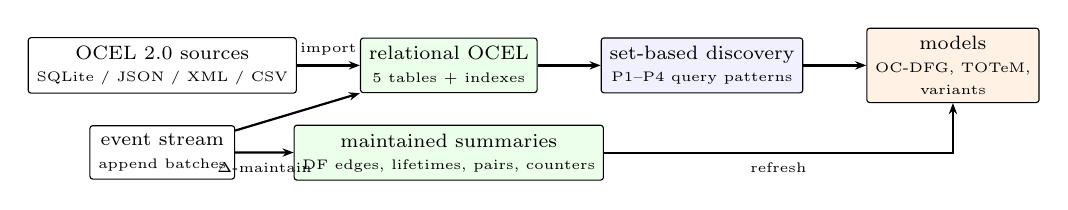
\begin{tikzpicture}[
  font=\scriptsize,
  box/.style={draw, rounded corners=1pt, align=center, inner sep=3pt, minimum height=14pt},
  store/.style={box, fill=green!8},
  comp/.style={box, fill=blue!6},
  outbox/.style={box, fill=orange!10},
  arr/.style={-{Stealth[length=4pt]}, thick}
]
\node[box] (src) {\ocel sources\\ \tiny SQLite / JSON / XML / CSV};
\node[store, right=8mm of src] (db) {relational OCEL\\ \tiny 5 tables + indexes};
\node[store, below=4mm of db] (state) {maintained summaries\\ \tiny DF edges, lifetimes, pairs, counters};
\node[comp, right=8mm of db] (sql) {set-based discovery\\ \tiny P1--P4 query patterns};
\node[outbox, right=8mm of sql] (models) {models\\ \tiny OC-DFG, TOTeM,\\ \tiny variants};
\node[box, below=4mm of src] (stream) {event stream\\ \tiny append batches};
\draw[arr] (src) -- node[above]{\tiny import} (db);
\draw[arr] (db) -- (sql);
\draw[arr] (sql) -- (models);
\draw[arr] (stream) -- node[below, sloped]{\tiny $\Delta$-maintain} (state);
\draw[arr] (stream) -- (db.south west);
\draw[arr] (state) -| node[below, pos=0.25]{\tiny refresh} (models.south);
\end{tikzpicture}
\caption{\sys architecture. Discovery runs as SQL inside the engine; appends maintain summary tables from which models are refreshed without scanning the log.}
\label{fig:arch}
\end{figure}

\subsection{Schema}
\label{sec:schema}

\sys stores a log in five normalized tables:

\begin{lstlisting}[caption={The \sys schema (attribute columns are discovered at import time; abbreviated).},label={lst:schema}]
CREATE TABLE events (
  event_id VARCHAR PRIMARY KEY,
  activity VARCHAR NOT NULL,
  timestamp_unix BIGINT NOT NULL
  /* + one column per event attribute */);
CREATE TABLE objects (
  obj_id VARCHAR PRIMARY KEY,
  obj_type VARCHAR NOT NULL
  /* + one column per object attribute */);
CREATE TABLE event_object (
  event_id VARCHAR NOT NULL, obj_id VARCHAR NOT NULL,
  qualifier VARCHAR, PRIMARY KEY (event_id, obj_id));
CREATE TABLE object_attribute_history (
  obj_id VARCHAR NOT NULL, timestamp_unix BIGINT NOT NULL,
  /* attribute columns */ PRIMARY KEY (obj_id, timestamp_unix));
CREATE TABLE object_relations (
  source_obj_id VARCHAR NOT NULL, target_obj_id VARCHAR NOT NULL,
  qualifier VARCHAR, PRIMARY KEY (source_obj_id, target_obj_id));
\end{lstlisting}

The schema mirrors Definition~\ref{def:ocel}: \texttt{events} and \texttt{objects} carry the functions $\mathit{act}$, $\mathit{time}$, $\mathit{type}$; \texttt{event\_object} is $R$ with qualifiers; \texttt{object\_relations} is $R_O$; \texttt{object\_attribute\_history} captures \ocel's dynamic object attributes. Three design decisions matter for performance. (i)~\emph{Attribute pivoting}: instead of storing attributes as JSON blobs or key--value pairs (as in the \ocel SQLite serialization, which spreads attributes over one table per event/object type), attributes become real columns discovered at import time, so analysts write plain SQL and the engine prunes unused columns. (ii)~\emph{Surrogate-free keys}: the natural identifiers are the keys, and secondary indexes on \texttt{event\_object(obj\_id)}, \texttt{event\_object(event\_id)}, \texttt{objects(obj\_type)}, and \texttt{events(timestamp\_unix)} cover all access paths used by discovery. (iii)~\emph{Single-file persistence}: the populated database is the cache; re-opening it costs milliseconds, whereas every in-memory tool re-parses the source log on every session (Section~\ref{sec:eval-real}).

Import supports all three \ocel serializations (SQLite, JSON, XML) plus CSV, with a bulk path (attach/Arrow ingestion) and a constant-memory streaming path for sources larger than a configurable threshold; referential violations (dangling links, duplicate keys) are optionally dropped during import.

\subsection{Query Patterns}
\label{sec:patterns}

Across the algorithms in Section~\ref{sec:artifacts}, four relational patterns recur:

\begin{description}
\item[P1 Per-object adjacency.] Consecutive event pairs within each object's trace, computed by window functions partitioned by object: the basis of directly-follows edges, trace starts/ends, and event-object graph edges.
\item[P2 Lifetime summarization.] Per-object interval aggregates $(\min,\max)$ over the E2O join: the basis of all temporal classification, computed \emph{before} any pairwise join (eager aggregation).
\item[P3 Co-occurrence pairs.] The connected-objects relation $\sim$, obtained by a self-join of \texttt{event\_object} on \texttt{event\_id}, deduplicated, united with $R_O$: the basis of TOTeM's log cardinalities and temporal relations and of variant extraction.
\item[P4 Type-cardinality counting.] Grouped counts of objects per type per event (or per neighborhood), cross-joined with the type domain to account for zero counts: the basis of EC/LC statistics.
\end{description}

Every artifact in Section~\ref{sec:artifacts} is a composition of P1--P4 followed by a small aggregation, and Section~\ref{sec:incremental} shows that exactly these patterns are also the incrementally maintainable state. The patterns compile to scans, hash joins, sorts, and hash aggregates---operators for which analytical engines provide parallel, out-of-core implementations. \sys thereby inherits multi-core execution and graceful spilling without any bespoke infrastructure.

\section{Discovery in SQL}
\label{sec:algorithms}

\subsection{OC-DFG: Window Functions vs.\ Self-Joins}
\label{sec:ocdfg-sql}

The textbook SQL formulation of ``$b$ directly follows $a$ for object $o$''---used by prior SQL-based (single-case) process mining~\cite{schonig2016sql}---is a self-join with a \texttt{NOT EXISTS} witness check: event pairs of the same object with no event in between. Per object of trace length $L$ this enumerates $O(L^2)$ candidate pairs and checks up to $O(L)$ witnesses each; the dominant cost is $\Theta(\sum_o L_o^2)$ before grouping. \sys instead computes P1 with a single window pass:

\begin{lstlisting}[caption={OC-DFG core (P1). Three further aggregations over the same CTE yield node frequencies and start/end counts.},label={lst:ocdfg}]
WITH event_sequence AS (
  SELECT e.event_id, e.activity, o.obj_id, o.obj_type,
         LAG(e.activity)  OVER w AS prev_activity,
         LEAD(e.activity) OVER w AS next_activity
  FROM events e
  JOIN event_object eo ON e.event_id = eo.event_id
  JOIN objects o       ON eo.obj_id  = o.obj_id
  WINDOW w AS (PARTITION BY eo.obj_id
               ORDER BY e.timestamp_unix, e.event_id))
SELECT obj_type, activity AS src, next_activity AS tgt,
       COUNT(*) AS weight
FROM event_sequence WHERE next_activity IS NOT NULL
GROUP BY ALL;
\end{lstlisting}

The window formulation costs one sort (or hash partition) of the $m$ E2O rows, $O(m \log m)$, independent of trace length, and start/end counts fall out of the same CTE via \texttt{prev\_activity IS NULL} / \texttt{next\_activity IS NULL}. Section~\ref{sec:eval-ablation} measures the gap between the two formulations on identical data; both produce identical graphs (tested).

\subsection{TOTeM: Eager Lifetime Aggregation}
\label{sec:totem-sql}

TOTeM discovery decomposes into five queries over the schema: (1)~activity/type mappings, (2)~related type pairs, (3)~event cardinalities via P4, (4)~log cardinalities via P3+P4, and (5)~temporal relations via P2+P3. The performance-critical phase is (5). A literal transcription of the in-memory algorithm iterates over connected object pairs and, for each pair, inspects both objects' events---in SQL, a join of the pair relation with \emph{all events of both objects}, producing $\sum_{(o_1,o_2)\in\sim} |\mathit{ev}(o_1)|\cdot|\mathit{ev}(o_2)|$ intermediate rows before aggregating interval bounds per pair (\emph{lazy aggregation}). \sys instead applies eager aggregation~\cite{yan1995eager}: P2 first reduces every object to one row $(\mathit{obj}, \mathit{type}, \min t, \max t)$, after which the pair join touches exactly $|{\sim}|$ rows, and the interval classification is a constant-time CASE expression per pair:

\begin{lstlisting}[caption={TOTeM temporal relations (P2+P3, abbreviated): lifetimes are aggregated before the pair join; the four CASE sums classify interval containment and overlap order.},label={lst:totem}]
WITH lifetimes AS (
  SELECT o.obj_id, o.obj_type,
         MIN(e.timestamp_unix) AS min_t,
         MAX(e.timestamp_unix) AS max_t
  FROM objects o
  JOIN event_object eo ON o.obj_id = eo.obj_id
  JOIN events e ON eo.event_id = e.event_id
  GROUP BY o.obj_id, o.obj_type),
all_conn AS (/* P3: e2o self-join UNION o2o */)
SELECT ls.obj_type, lt.obj_type, COUNT(*),
  SUM(CASE WHEN lt.min_t <= ls.min_t
            AND ls.max_t <= lt.max_t THEN 1 ELSE 0 END), ...
FROM all_conn ac
JOIN lifetimes ls ON ac.src_obj = ls.obj_id
JOIN lifetimes lt ON ac.tgt_obj = lt.obj_id
GROUP BY ls.obj_type, lt.obj_type;
\end{lstlisting}

With $\bar{L}$ the mean trace length, eager aggregation reduces the intermediate from $\Theta(|{\sim}|\,\bar{L}^2)$ to $\Theta(m + |{\sim}|)$ rows (Table~\ref{tab:complexity}).

\begin{table}
\caption{Dominant intermediate sizes of the naive vs.\ optimized formulations ($m=|R|$, $\bar{L}$ mean trace length, $\sim$ connected object pairs).}
\label{tab:complexity}
\small
\begin{tabular}{lll}
\toprule
Phase & Naive & Optimized \\
\midrule
DF extraction & $\Theta(\sum_o L_o^2)$ pairs $\times$ $O(L_o)$ checks & $O(m \log m)$ \\
Temporal rel. & $\Theta(|{\sim}|\,\bar{L}^2)$ & $\Theta(m + |{\sim}|)$ \\
\bottomrule
\end{tabular}
\end{table} The same rewrite applies to log cardinalities, where the count of connected objects per type is aggregated per source object before bucketing into $\{0, 1, >1\}$. Phase~(3) computes, for every event and type, the number of participating objects of that type (P4) and buckets them per source--target type pair; the final model assembly (selecting the most precise label per type pair under $\tau$) operates on a few hundred aggregate rows in Python, unchanged from the reference implementation~\cite{liss2024totem}.

\subsection{Variants: Hybrid Set-Based/Graph Processing}
\label{sec:variants-sql}

Variant analysis is the least SQL-friendly of the three tasks because its final step---grouping process executions by typed graph isomorphism---has no relational formulation. \sys splits the task: execution extraction (leading-object neighborhoods or connected components over P3) and the materialization of per-execution event multisets and adjacency structures run as set-based SQL; the grouping step offers a spectrum of strategies, from a purely relational multiset signature (sound for grouping only up to label multiplicity), over Weisfeiler--Lehman hashing~\cite{wl2011}, to exact VF2 isomorphism~\cite{vf2} refinement of WL buckets. The hybrid keeps the data-intensive part in the engine and the combinatorial part on aggressively reduced inputs. As variants are not the focus of this paper, we evaluate only the end-to-end effect (Section~\ref{sec:eval-real}) and refer to~\cite{adams2022variants} for the semantics.

\section{Incremental Discovery}
\label{sec:incremental}

Operational logs grow continuously. In all published OCPM tools, refreshing a model after new events arrive requires re-importing the log and recomputing from scratch---$O(n)$ work per refresh. \sys instead treats the aggregates behind each model as materialized views and maintains them under \emph{event-batch appends}: a batch $B$ of new events with their E2O links (an event arrives together with its links), possibly new objects, and new O2O relations.

\subsection{Maintained State}

For the OC-DFG, \sys maintains the edge-weight table, per-type activity frequencies, start/end counts, and a per-object head/tail state (first/last activity, last timestamp). For TOTeM, it maintains object lifetimes, the connected-pair relation with each pair's interval classification stored as a 4-bit mask, per-source-object connection counts by target type, additive EC counters, and the (monotone) activity/type and type-pair relations. Both states live in ordinary tables inside the same database, so maintenance steps are themselves set-based SQL (\texttt{INSERT \ldots ON CONFLICT DO UPDATE}).

\subsection{Delta Propagation}

\paragraph{OC-DFG} Under the natural assumption that appends respect per-object order (each object's new events come after its previously seen events), the new directly-follows edges of batch $B$ are exactly (i)~adjacent pairs \emph{within} $B$ per object---computed by the same window query as Listing~\ref{lst:ocdfg} restricted to $B$---plus (ii)~one \emph{bridge} edge per touched known object, from its stored last activity to its first new activity. End counts move from each touched object's old last activity to its new one; start counts grow only for newly active objects. The append cost is $O(|B| \log |B|)$ plus one upsert per touched object, independent of $n$; out-of-order appends are detected and rejected.

\paragraph{TOTeM} No ordering assumption is needed: every maintained TOTeM aggregate is order-independent. Lifetimes are upserted with $\min/\max$. EC counters are strictly additive because events are immutable once their links arrived. The subtle part is the pair classification: appending events can \emph{grow} the lifetime interval of a known object, which may reclassify \emph{every} pair incident to it. \sys therefore recomputes the classification mask exactly for the \emph{affected pairs}---new pairs (first co-occurrence in $B$, or O2O relations whose endpoints became active) and existing pairs incident to an object whose interval changed---via one join against the lifetime table. Model refresh then aggregates the summary tables only ($O(|{\sim}| + |O|)$, no scan of \texttt{events} or \texttt{event\_object}), and reuses the unchanged label-selection logic.

\begin{proposition}[Equivalence]
\label{prop:equiv}
After any sequence of valid batch appends, the OC-DFG (resp.\ TOTeM model) materialized from the maintained state equals the result of the full SQL recomputation of Section~\ref{sec:algorithms} over the accumulated log.
\end{proposition}

\begin{proof}[Proof sketch]
For the OC-DFG, ordered appends imply that each object's trace is a concatenation of its per-batch subtraces; adjacent pairs are either within one batch (case~i) or bridge consecutive batches (case~ii), and first/last elements evolve as maintained. For TOTeM, each maintained table equals the corresponding subexpression of the full query: lifetimes and EC counters by distributivity of $\min/\max/\mathrm{count}$ over unions, the pair relation because connectivity is monotone, and masks because they are recomputed from current lifetimes exactly for the pairs whose inputs changed---a pair not incident to a changed lifetime retains a valid mask. The property is additionally enforced by tests that replay real and synthetic logs in batches and assert equality after every batch.
\end{proof}

The per-batch maintenance cost is $O(|B|\log|B| + |\Delta{\sim}| + |{\sim_{\mathit{aff}}}|)$ where $\Delta{\sim}$ are new pairs and ${\sim_{\mathit{aff}}}$ the pairs incident to interval changes---in particular, independent of the number of events accumulated so far. Section~\ref{sec:eval-inc} confirms that maintenance plus refresh is orders of magnitude cheaper than recomputation and stays flat as the log grows.

\section{Experimental Evaluation}
\label{sec:eval}

We evaluate five questions.
\textbf{RQ1}: How does \sys scale with log size compared to in-memory OCPM (Section~\ref{sec:eval-scaling})?
\textbf{RQ2}: How much do the two query rewrites of Section~\ref{sec:algorithms} contribute (Section~\ref{sec:eval-ablation})?
\textbf{RQ3}: What does incremental maintenance save over recomputation (Section~\ref{sec:eval-inc})?
\textbf{RQ4}: Does \sys deliver under a hard memory budget (Section~\ref{sec:eval-mem})?
\textbf{RQ5}: How do storage footprint and end-to-end times compare on real logs (Section~\ref{sec:eval-real})?

\subsection{Setup}
\label{sec:eval-setup}

\paragraph{Environment}
All experiments run on a 4-core Intel Xeon @\,2.10\,GHz with 15\,GB RAM and local SSD, Linux, Python 3.11, DuckDB 1.5.3, Polars 1.41, pm4py 2.7.22. Every measurement executes in a fresh process; we report wall-clock time of the discovery computation itself (data loading reported separately where relevant) and the peak resident set size of the process. Runs are repeated three times up to $3{\cdot}10^5$ events (we report medians; variance is below 5\%) and once above. The timeout is 600\,s.

\paragraph{Baselines}
(i)~\emph{Polars}: the in-memory reference implementations of totem-tool, which already use a columnar dataframe engine and are therefore a strong baseline---they represent the state of practice of dedicated in-memory OCPM code. (ii)~\emph{pm4py}~\cite{pm4py}, the most widely used OCPM library, for OC-DFG discovery (pm4py implements no TOTeM). All three implementations of each algorithm produce identical models (verified).

\paragraph{Real logs}
We use the three public \ocel logs of Table~\ref{tab:datasets}: a container logistics process, a procure-to-pay (P2P) process, and the order management process.

\begin{table}
\caption{Real \ocel logs and their storage footprint (MB) in the three \ocel serializations vs.\ the \sys database.}
\label{tab:datasets}
\small
\setlength{\tabcolsep}{3.4pt}
\begin{tabular}{lrrrr|rrrr}
\toprule
 & & & & & \multicolumn{4}{c}{size [MB]} \\
Log & $|E|$ & $|O|$ & $|R|$ & types & JSON & XML & SQLite & \sys \\
\midrule
Logistics & 35,372 & 13,882 & 74,272 & 7 & 10.0 & 13.4 & 23.0 & \textbf{2.4} \\
P2P & 14,671 & 9,543 & 35,927 & 7 & 14.3 & 18.4 & 13.7 & \textbf{2.6} \\
Orders & 21,008 & 10,840 & 147,385 & 6 & 12.6 & 15.2 & 36.6 & \textbf{3.2} \\
\bottomrule
\end{tabular}
\end{table}

\paragraph{Synthetic logs}
The public logs are tiny by database standards. For controlled scaling we built a set-based generator that synthesizes \ocel logs \emph{inside} the engine (no Python row loops; $10^7$ events in under two minutes): $K{=}3$ object types form a hierarchy (e.g., order--item--package), every object runs a 10-event lifecycle, children start within their parent's lifetime, 30\% of child events also reference the parent (creating shared events and type interaction), and child--parent links are mirrored in O2O relations. All randomness is hash-based and seeded, so every configuration is exactly reproducible. We scale the number of objects to obtain $3{\cdot}10^4$--$10^7$ events.

\subsection{RQ1: Scalability}
\label{sec:eval-scaling}

\begin{figure*}
\centering
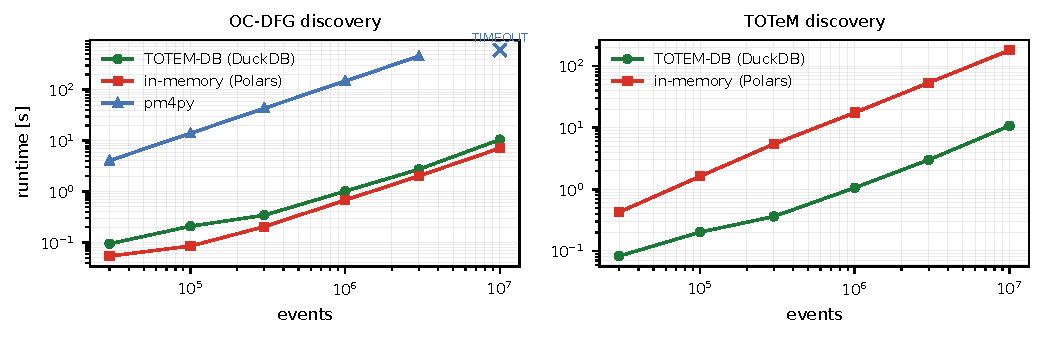
\includegraphics[width=0.85\textwidth]{figures/fig_scaling.pdf}
\caption{Discovery runtime over synthetic log size (log--log). $\times$ marks a failed run at its budget.}
\label{fig:scaling}
\end{figure*}

\begin{figure*}
\centering
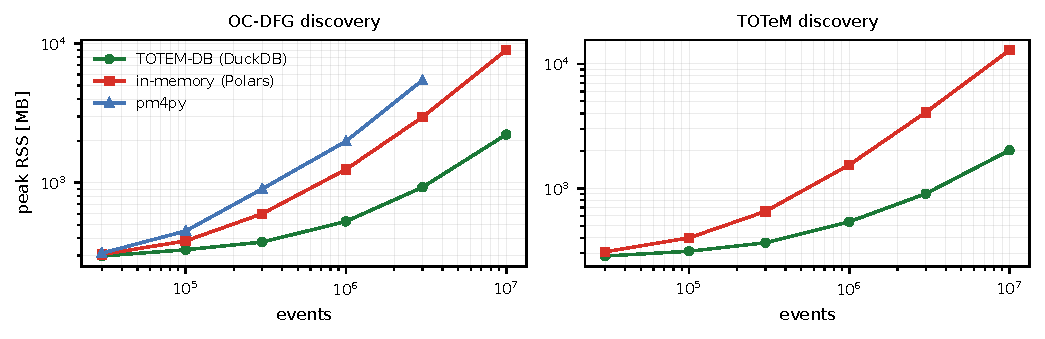
\includegraphics[width=0.85\textwidth]{figures/fig_scaling_memory.pdf}
\caption{Peak process RSS for the runs of Figure~\ref{fig:scaling}.}
\label{fig:scaling-mem}
\end{figure*}

Figure~\ref{fig:scaling} shows discovery runtimes from $3{\cdot}10^4$ to $10^7$ events; Figure~\ref{fig:scaling-mem} the corresponding peak memory. Three observations.

First, \emph{\sys scales linearly and stays interactive}: OC-DFG and TOTeM discovery over $10^7$ events take 10.5\,s and 10.7\,s respectively. pm4py, the most widely used OCPM implementation, is two orders of magnitude slower throughout (e.g., OC-DFG at $10^6$ events: 148\,s vs.\ 1.0\,s) and exceeds the 600\,s timeout at $10^7$ events.

Second, \emph{the gap to dedicated in-memory code depends on the algorithm's shape}. For the OC-DFG---essentially one grouped aggregation---the Polars baseline is marginally faster on the discovery step itself (7.1\,s vs.\ 10.5\,s at $10^7$), confirming that \sys's window-function plan is competitive with hand-written columnar code. For TOTeM, whose pair-classification step in-memory iterates over object pairs in Python, \sys is $17\times$ faster at $10^7$ events (10.7\,s vs.\ 180.6\,s) with the gap widening with size.

Third, \emph{the in-memory architecture pays hidden costs that \sys avoids}. The dataframe baseline must first materialize the log in RAM---21.9\,s of loading at $10^7$ events before the first query, against milliseconds to open the \sys database---and its footprint grows to 9.0\,GB (OC-DFG) and 12.9\,GB (TOTeM) at $10^7$ events, 86\% of the machine's RAM: the next log-size step is out of reach, exactly where Figure~\ref{fig:scaling-mem} shows \sys at 2.0--2.2\,GB, and RQ4 shows \sys completing the same workload in 500\,MB.
\subsection{RQ2: Effect of the Query Rewrites}
\label{sec:eval-ablation}

\begin{figure*}
\centering
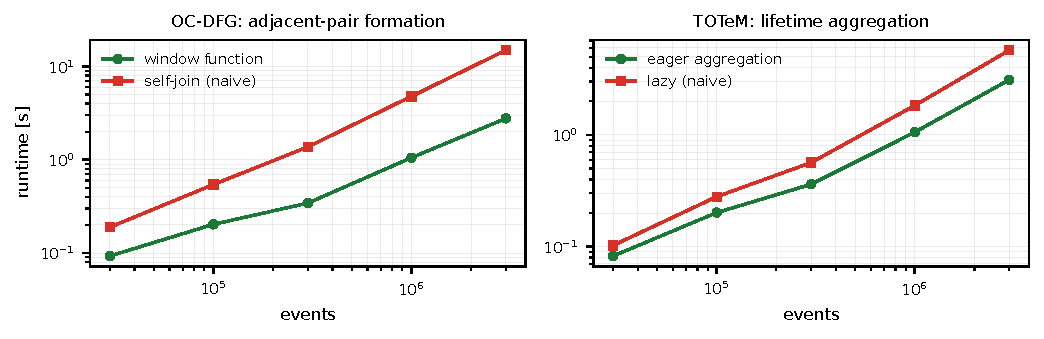
\includegraphics[width=0.85\textwidth]{figures/fig_ablation.pdf}
\caption{Optimized vs.\ naive SQL formulations over log size (trace length $L{=}10$).}
\label{fig:ablation}
\end{figure*}

\begin{figure*}
\centering
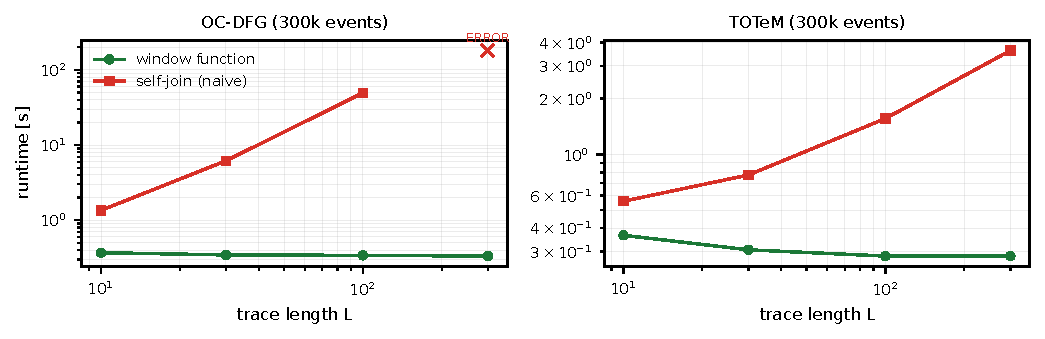
\includegraphics[width=0.85\textwidth]{figures/fig_ablation_tracelen.pdf}
\caption{Optimized vs.\ naive formulations over trace length $L$ at a fixed $3{\cdot}10^5$ events.}
\label{fig:ablation-tracelen}
\end{figure*}

Figure~\ref{fig:ablation} compares the optimized formulations against their naive counterparts on identical data (both produce identical models; enforced by tests). With short traces ($L{=}10$), the window-function OC-DFG is already $5.4\times$ faster than the self-join formulation at $3{\cdot}10^6$ events (2.8\,s vs.\ 14.9\,s) while using $6.6\times$ less memory (0.9\,GB vs.\ 6.1\,GB)---the quadratic candidate space materializes as memory pressure before it dominates runtime. Eager lifetime aggregation accelerates TOTeM by $1.8\times$ at this trace length.

The decisive variable is trace length (Figure~\ref{fig:ablation-tracelen}): holding the event count fixed at $3{\cdot}10^5$ and growing $L$ from 10 to 300 leaves the optimized formulations essentially flat, while the naive intermediates grow as predicted by Table~\ref{tab:complexity}.
% FILL:tracelen
% FILL:RQ3
\subsection{RQ4: Discovery under a Memory Budget}
\label{sec:eval-mem}

\begin{table}
\caption{Discovery over the $10^7$-event log under hard memory budgets. \sys budgets bound the engine's buffer pool (spilling to disk); the in-memory baseline gets a 4\,GB address-space limit.}
\label{tab:memory}
\small
\begin{tabular}{llrrr}
\toprule
Algorithm & Engine & Budget & Time [s] & Peak RSS \\
\midrule
\multirow{4}{*}{OC-DFG}
 & \sys & 4\,GB & 10.6 & 2.2\,GB \\
 & \sys & 1\,GB & 11.7 & 1.3\,GB \\
 & \sys & 500\,MB & 15.4 & 0.85\,GB \\
 & Polars & 4\,GB & \multicolumn{2}{c}{out of memory} \\
\midrule
\multirow{4}{*}{TOTeM}
 & \sys & 4\,GB & 11.1 & 2.3\,GB \\
 & \sys & 1\,GB & 15.5 & 1.6\,GB \\
 & \sys & 500\,MB & 22.1 & 0.99\,GB \\
 & Polars & 4\,GB & \multicolumn{2}{c}{out of memory} \\
\bottomrule
\end{tabular}
\end{table}

Scalability in RQ1 was bounded by the machine's 15\,GB of RAM. Table~\ref{tab:memory} probes behavior when memory is scarce: we repeat the $10^7$-event experiment with the engine's memory limit set to 4\,GB, 1\,GB, and 500\,MB (with a disk spill directory), and give the in-memory baseline an equivalent 4\,GB address-space budget. \sys completes every configuration: constraining the budget by $8\times$ (4\,GB${\to}$500\,MB) slows OC-DFG discovery by only $1.5\times$ and TOTeM by $2.0\times$, the signature of out-of-core operators that degrade gracefully rather than fail. The in-memory implementations---which need 9.0--12.9\,GB for this log (Figure~\ref{fig:scaling-mem})---abort with out-of-memory errors three seconds into loading. Bounded-memory execution is not a corner case: it is precisely the situation of an analyst's laptop or a multi-tenant analysis service, and it is where the architectural difference is qualitative, not quantitative.
\subsection{RQ5: Real Logs, Import, and Storage}
\label{sec:eval-real}

\begin{figure*}
\centering
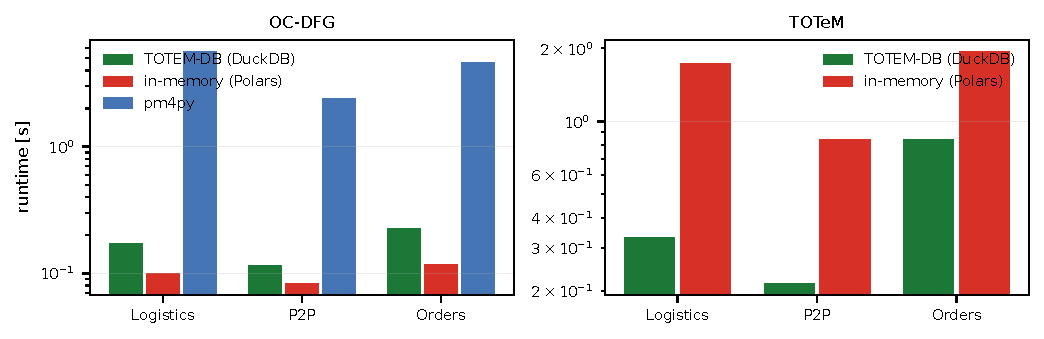
\includegraphics[width=0.85\textwidth]{figures/fig_real.pdf}
\caption{Discovery runtime on the three real \ocel logs (log scale).}
\label{fig:real}
\end{figure*}

\paragraph{Discovery}
Figure~\ref{fig:real} confirms the synthetic findings on real data: against pm4py, \sys discovers OC-DFGs $14$--$33\times$ faster (e.g., 0.17\,s vs.\ 5.6\,s on the logistics log); against the Polars implementations, TOTeM discovery is $2.3$--$5.2\times$ faster, while the OC-DFG aggregation is comparable. Variant analysis behaves as predicted in Section~\ref{sec:variants-sql}: where the exact-isomorphism step is tractable, the hybrid \sys pipeline matches or beats the in-memory implementation (logistics: 0.46\,s vs.\ 0.96\,s for 16 variants; P2P: 5.1\,s vs.\ 4.9\,s for 444 variants); on the order-management log, whose order-centered process executions form very large connected graphs, \emph{both} implementations exhaust memory in the exact-isomorphism step---the bottleneck is combinatorial, not data movement, and \sys's coarser relational grouping strategies (multiset signatures, WL hashing) remain available as approximations.

\paragraph{Import and re-analysis}
Parsing the JSON serialization costs 1.0--1.3\,s (Polars) and 1.4--2.8\,s (\sys, including index construction) on these logs---but the in-memory pipeline pays its cost on \emph{every} session, whereas the \sys database is the persistent store: re-opening it costs 25--30\,ms, after which discovery runs directly. For the recurring analyses that dominate practice (daily refreshes, dashboards, interactive exploration), the relational architecture eliminates the dominant fixed cost. At $10^7$ events this difference is 22\,s per session (RQ1).

\paragraph{Storage}
Table~\ref{tab:datasets} shows a further operational benefit: the typed, columnar \sys database is $4$--$11\times$ smaller than any \ocel interchange serialization of the same logs (e.g., logistics: 2.4\,MB vs.\ 10.0--23.0\,MB), making the database the cheapest representation to retain as well as the fastest to analyze.

\subsection{Discussion and Limitations}
\label{sec:eval-discussion}

\sys's incremental layer assumes events arrive with their object links, and the OC-DFG maintainer additionally assumes per-object append order (violations are detected, and the state can be re-bootstrapped in one pass). Attribute pivoting assumes a bounded attribute vocabulary; logs with thousands of distinct attribute keys would need a hybrid layout. Our SQL relies only on standard window functions, grouped aggregation, and upserts and ports to other engines with minor dialect changes, but our measurements cover DuckDB; a cross-engine study (including a client--server setting where the log never leaves the operational warehouse) is future work. Finally, the isomorphism step of variant analysis remains outside the relational engine; its cost dominates exactly when process executions are large.

\section{Conclusion}
\label{sec:conclusion}

Object-centric event data is relational; \sys shows that object-centric process discovery can and should be relational too. Expressing OC-DFG, TOTeM, and variant discovery over a normalized \ocel schema---with window-function adjacency and eager interval aggregation as the two decisive rewrites---yields discovery that is faster than specialized in-memory implementations, scales beyond memory through out-of-core execution, and, via incremental view maintenance of the underlying summaries, supports always-fresh models over growing logs at a per-batch cost independent of log size. We see two natural next steps: extending the maintained-summary approach to further OCPM artifacts (object-centric Petri nets, conformance statistics), and pushing the variant-isomorphism frontier further into the engine via relational graph-canonization primitives.

\begin{acks}
The author thanks the PADS group at RWTH Aachen University.
\end{acks}

\bibliographystyle{ACM-Reference-Format}
\bibliography{references}

\end{document}
